\documentclass{article}
\usepackage[margin=3cm]{geometry}
\usepackage[backend=biber, style=authoryear, urldate=long, url=true, doi=true, natbib=true]{biblatex}
\usepackage{graphicx, wrapfig}

\addbibresource{it_wissensmanagement.bib}
\frenchspacing
\title{Wissensmanagement IT}
\author{Nikolai Furmanczak}

\begin{document}
\section*{Wissensmanagement in der IT}
Die IT, unabhängig welche Teildisziplin, gehört wohl unumstritten zu den Branchen die am schnelllebigsten sind. Dies hat sich insbesondere in den Themen Cloud-Computing oder Künstliche Inteligenz (KI) in den letzten Jahren deutlich wiedergespiegelt. Neben der schnelligkeit tendiert die IT aber auch zu einer besonderen komplexität. Infrastukturen bestehen immer aus immer mehr Komponenten und in einem Softwareprojekt gibt es immer mehr Abhängigkeiten zu anderen Frameworks oder Bibiliotheken. Vor allem JavaScript Entwickler werden den letzten Punkt kennen. Diese beiden Punkte - komplexität und schnelligkeit - führen zu einer immer größer werdenen Flut an Informationen und Wissen die  bewältigt müssen. Damit wichtiges Wissen nicht verloren geht und auch innerhalb einer Firma geteilt wird, sollten sich Unternehmen aber auch Manager mit dem Thema Wissensmanagement beschäftigen. Um direkt eins vorweg zu nehmen: Das alleinige pflegen eines Wikis zählt nicht als Wissensmanagement.
\subsubsection*{Wissen versus Informationen}
Bevor wir uns mit dem Thema Wissensmanagement befassen, sollten wir den Begriff "Wissen" definieren. Leider gibt es in der Literatur keine einheitliche Definition \parencite{ReinmannRothmeierMandl2000}. Die Definition hängt vielmehr vom Blickwinkel auf das Thema ab. Nach Fischer und Wewer entsteht Wissen durch einem Lernprozess bei dem Informationen interpretiert und verarbeitet werden \parencite*[p. 2]{FischerWewer2021}. Hieran erknenne wir das es einen Unterschied zwischen Informationen und Wissen gibt. Informationen sind die Vorstufe zu Wissen. In der Praxis werden Wissen und Informationen fälschlicherweise oft gleichgesetzt. Modelle wie die Wissenstreppe (siehe Figure 1) von Klaus North verdeutlichen welche Schritte notwendig sind um Wissen zu erzeugen.   
\begin{wrapfigure}{r}{0.5\textwidth}
    \centering
    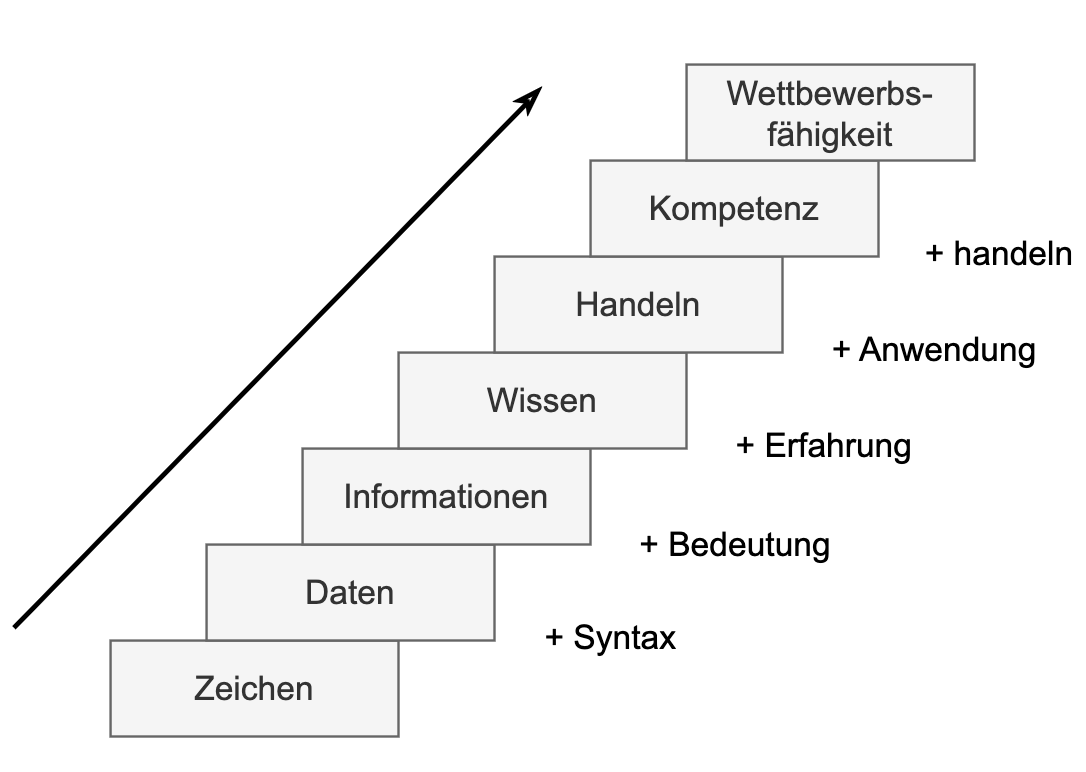
\includegraphics[width=0.5\textwidth]{images/wissenstreppe.png}
    \caption{Wissenstreppe}
    \label{fig:meinBild}
  \end{wrapfigure}
Aus der Wissenstreppe können wir grob entnehmen welche Benefits ein korrektes Wissensmanagement mit sich bringt: mehr kompetenz bei Mitarbeitern, verkürzte einarbeitungszeit und gesteigerte Motivation durch die erweiterte Wissensbasis \parencite{NorthSchmidt2004}. Durch Wissensaustausch, bessere (interne) Kommunikation steigt auch die Kundenzufriedenheit \parencite{NorthSchmidt2004}
\subsubsection*{Implizites und Explizites Wissen} 
Wissen kann in verschiedene kategorien eingeteilt werden. Die häufigste, und vielleicht auch wichtigste, ist in implizites und explizites Wissen. Im Gegensatz zum expliziten Wissen kann implizites Wissen nicht (leicht) vom Träger weitergegeben werden \parencite[p. 2]{FischerWewer2021}. Deswegen wird implizites auch verborgenes Wissen genannt. Es baut hauptsächlich auf Erfahrung auf. Das klassische Beispiel für Explizites Wissen sind schriftliche Dokumentationen oder Anleitungen. Implizites Wissen zeigt sich beispielweise beim debuggen eines schwierigen Problems oder planung eines komplexen Projektes.
\printbibliography
\end{document}
